\documentclass[12pt,a4paper]{report}
\usepackage[a4paper,
    left=1.25in,
    right=1in,
    top=1in,
    bottom=1in]{geometry} % Required for inserting images
\usepackage{fullpage}
\usepackage{mathptmx}
\usepackage{titletoc}
\usepackage[titles]{tocloft}
\usepackage{booktabs}   % For professional table formatting
\usepackage{array}      % For enhanced table control
\usepackage{siunitx}    % For proper number formatting
%\usepackage{geometry}   % To adjust page margins
\usepackage{float}

\usepackage{lipsum}
\usepackage{acronym}
\usepackage{graphicx}
% Add to your main document preamble
\usepackage{tikz}
\usetikzlibrary{shapes,arrows,fit,positioning}
\graphicspath{ {./images/} }
\usepackage{pgfgantt}

% Line spacing
\usepackage{setspace}  
\onehalfspacing  % or use \singlespacing or \doublespacing as needed

% Paragraph spacing
\setlength{\parskip}{0.75em}  % space between paragraphs
\setlength{\parindent}{0pt}   % no indentation (you already have this)

% Custom font sizes for headings
\usepackage{sectsty} % to customize section font sizes

% Normal text font size is already 12pt (from documentclass)

% Normal heading style (like \textbf 12pt) - redefine \normalfont
\renewcommand\normalsize{\fontsize{12}{14}\selectfont} % 12pt font with 14pt baseline skip

% Section headings (14pt)
\sectionfont{\fontsize{14}{16}\selectfont\bfseries} 

% Subsection headings (optional, keep smaller)
\subsectionfont{\fontsize{12}{14}\selectfont\bfseries}

% Chapter (main heading) size (16pt bold centered)
\usepackage{titlesec}
\titleformat{\chapter}[display]
  {\normalfont\bfseries\fontsize{16}{18}\selectfont\centering}
  {\chaptername\ \thechapter}{1em}{}

\renewcommand*\contentsname{Table of Contents}

% Redefine the \numberline command for figures
\newlength{\mylen}
\renewcommand{\cftdotsep}{0.5}
\renewcommand{\cftfigpresnum}{\hspace*{-1.5em}\figurename\enspace}
\renewcommand{\cftfigaftersnum}{:}
\settowidth{\mylen}{\cftfigpresnum\cftfigaftersnum}
\addtolength{\cftfignumwidth}{\mylen}


\renewcommand{\cftdotsep}{0.5}
\renewcommand{\cfttabpresnum}{\hspace*{-1.5em}\tablename\enspace}
\renewcommand{\cfttabaftersnum}{:}
\settowidth{\mylen}{\cfttabpresnum\cfttabaftersnum}
\addtolength{\cfttabnumwidth}{\mylen}


\titlecontents{chapter}
[5.5em] %5.3
{\smallskip}
{\contentslabel[\bfseries{\chaptername}~\thecontentslabel{:}]{5.5em}\textbf}%\thecontentslabel
{\hspace*{-5.5em}\textbf}% unnumbered chapters
{\titlerule*[0.35pc]{.}\contentspage}[\smallskip]%

\titlecontents{section}
[1.5em] % i
{\smallskip}
{\thecontentslabel\enspace}%\thecontentslabel
{\hspace*{-5.5em}}
{\titlerule*[0.35pc]{.}\contentspage}%]

\titlecontents{subsection}
[7.12em] %
{\smallskip}
{\thecontentslabel\enspace}%\thecontentslabel
{\hspace*{7.12em}}
{\titlerule*[0.35pc]{.}\contentspage}

\makeatletter
\renewcommand{\@makechapterhead}[1]{%\vspace*{50 pt}%
{\setlength{\parindent}{0pt}\normalfont
\bfseries\Huge\chaptername{\hspace*{0.25em}}\centering\thechapter{:}\ #1
\par\nobreak\vspace{16 pt}}}
\makeatother

\makeatletter
\renewcommand{\@makeschapterhead}[1]{%\vspace*{50 pt}%
{\setlength{\parindent}{0pt}\normalfont
\bfseries\Huge\centering\ #1
\par\nobreak\vspace{16 pt}}}
\makeatother

\title{Major}
\author{Mahan Sigdel}
\date{May 2025}

\setlength{\parindent}{0pt}

\begin{document}
\begin{titlepage}
    \thispagestyle{empty}
    \begin{center}
    
    \vspace*{\fill} % * makes latex to not ignore the command
    \vspace*{-1cm}
    {\large \textbf{TRIBHUVAN UNIVERSITY
}\par}
{\large \textbf{INSTITUTE OF ENGINEERING
}\par}
\vspace{8pt}
KATHMANDU ENGINEERING COLLEGE

KALIMATI,KATHMANDU
\vspace{24pt}

\begin{figure}[ht]
    \centering
    
\includegraphics[scale=0.45]{images/kec.png}
\end{figure}
\vspace{24pt}
{MINOR PROJECT PROPOSAL REPORT ON\par}
\vspace{14pt}
{\textbf{ `MODULAR BOT'}\par}

\vspace{14pt}
{BY\par}
\vspace{14pt}

{ ARAJ BAHADUR CHHETRI - KAT079BEI008\par}
{ PRASUN PAUDEL - KAT079BEI024\par}
{RASDEEP BAJRACHARYA - KAT079BEI026\par}
{VIDHAN KHANAL - KAT079BEI047\par}

\vspace{24pt}
{TO\par}
\vspace{14pt}
{DEPARTMENT OF ELECTRONICS, COMMUNICATION AND INFORMATION ENGINEERING\par}
{KATHMANDU, NEPAL\par}
{MAY , 2024\par}

    %\vspace*{\fill}

    \end{center}
\end{titlepage}

\pagenumbering{roman}

\chapter*{Acknowledgement}
\addcontentsline{toc}{chapter}{Acknowledgement}
\label{acknowledgement}
We would like to express our sincere gratitude to the Department of Electronics, Communication, and Information, Kathmandu Engineering College, for providing us with an opportunity to initiate our minor project as a part of a syllabus. And a special thanks goes to our supervisor, \textbf{Er. Ravi Poudel}, for assisting and aiding us in every possible way in this project. We are deeply thankful to the Project Coordinator, \textbf{Er. Dhawa Song Dong}. We would also like to mention a special note of thanks to the esteemed Head of the Department of Electronics, Communication, and Information, \textbf{Er. Suramya Dahal}. We would also like to extend our gratitude to every teacher of the Department of Electronics, Communication and Information, for their guidance.

%\chapter*{Abstract}
%\addcontentsline{toc}{chapter}{Abstract}
%\label{abstract}
%\lipsum[2-4]

\tableofcontents
\thispagestyle{empty}
\addtocounter{page}{-1}
\newpage

\listoffigures
\addcontentsline{toc}{chapter}{List of Figures}
\newpage

\listoftables
\addcontentsline{toc}{chapter}{List of Tables}
\newpage

\chapter*{List of Abbreviation}
\addcontentsline{toc}{chapter}{List of Abbreviation}
\label{abbreviation}
\begin{acronym}
 \acro{MPU:}{Motion Processing Unit}
 \acro{IMU:}{Inertial Measurement Unit}
 \acro{HCI:}{Human-Computer Interaction}
 \acro{DoF:}{Degrees of Freedom}
 \acro{VR:}{Virtual Reality}
 \acro{AR:}{Augmented Reality}
 \acro{PLA:}{Polylactic Acid}
 \acro{ESP:}{Espressif Systems}
 \acro{IoT:}{Internet of Things}
 \acro{VAR:}{Virtual Augmented Reality}
 \acro{MEMS:}{Micro-Electro-Mechanical Systems}
 \acro{DMP:}{Digital Motion Processor}
 \acro{TCP/IP:}{Transmission Control Protocol/Internet Protocol}
 \acro{CPU:}{Central Processing Unit}
 \acro{GPU:}{Graphics Processing Unit}
 \acro{Wi-Fi:}{Wireless Fidelity}
 \acro{RISC:}{Reduced Instruction Set Computer}
 \acro{IEEE:}{Institute of Electrical and Electronics Engineers}
 \acro{HTTP:}{Hypertext Transfer Protocol}
 \acro{IDE:}{Integrated Development Environment}
 \acro{API:}{Application Programming Interface}
 \acro{EEVEE:}{Enhanced Efficient Virtual Environment Engine}
 

\end{acronym}
\newpage

\pagenumbering{arabic}

\chapter{Introduction}
\label{introduction}
\section{Background Theory}
The rapid integration of robotics into healthcare environments is transforming traditional caregiving approaches. With rising demands for efficient patient management in hospitals, hostels, and elderly care centers, autonomous service robots are becoming an innovative solution. These robots, especially those capable of delivering medications and supplies, offer consistent, scheduled, and contactless services that reduce human error and free up valuable time for medical personnel.

Among the various robotic systems being developed, line-following robots have gained attention for their simplicity, reliability, and adaptability in structured indoor environments like hospital wards or dormitories with fixed bed layouts. These robots navigate by following predefined paths, typically using infrared (IR) sensors to detect contrasting lines on the floor. Such navigation is especially useful for environments where precise, repeatable routes are needed to deliver medication trays to specific beds.

The proposed system enhances this concept by introducing a three-compartment modular robot. The bottom compartment houses motion components, including motors, wheels, sensors, and batteries, making it the foundation for navigation and mobility. The middle compartment is dedicated to general storage, such as medical equipment, water, or additional medicine trays. The top compartment features a smart pill dispenser powered by a Raspberry Pi and a camera. This setup allows the robot to identify patients using facial recognition algorithms and dispense medicine according to a preset time schedule, minimizing the chances of human error and increasing medication adherence.

To ensure robust interaction and real-time tracking, the system can integrate wireless communication modules (e.g., Wi-Fi or Bluetooth) to connect with a central server or a mobile application. This allows healthcare providers to monitor the robot’s location, view pill dispensing logs, and modify schedules as needed. The use of AI in facial recognition and scheduling also paves the way for personalized patient care, enabling the robot to adapt to individual needs.

Modularity in the robot’s design adds another layer of practicality. Each compartment is detachable and independently upgradable, enabling easy maintenance, swift replacements, and the possibility of repurposing the robot for different tasks (e.g., food delivery, waste collection) by simply swapping modules. Lightweight yet durable materials like 3D-printed PLA or ABS plastic are ideal for building these components, ensuring comfort, stability, and structural integrity.

In the broader context, this project reflects the growing intersection of robotics, AI, and healthcare—a convergence that is expected to redefine service delivery in hospitals. By aligning routine medical tasks with intelligent automation, such systems not only improve efficiency but also offer a glimpse into the future of compassionate, technology-driven patient care.

\vspace{1.5\baselineskip} 

\section{Problem Statement}
Modern healthcare systems—particularly in resource-constrained settings such as public hospitals, mass hostels, and elderly care facilities—face ongoing challenges in ensuring timely, consistent, and personalized delivery of medication. Relying on human staff for routine tasks such as distributing pills or tracking medication schedules often results in inefficiencies, human error, and missed doses, especially during peak workloads or emergencies. While existing medical robots offer partial automation, they are typically expensive, non-modular, or dependent on proprietary software, limiting their adaptability and scalability in practical environments.

Furthermore, most delivery bots lack intelligent interaction capabilities. They often depend solely on line-following navigation without integrating patient identification, flexible routing, or automated scheduling, making them unsuitable for truly personalized or responsive care. Pill-dispensing mechanisms in these systems are also generally basic, lacking integration with facial recognition, scheduling, or patient feedback mechanisms.

This project addresses these limitations by developing a low-cost, modular, and intelligent line-following medical assistant robot equipped with a smart pill dispensing system. The robot combines real-time navigation, multi-compartment storage, and a top-mounted AI-driven module featuring a Raspberry Pi and camera for facial recognition and time-based pill dispensing. The modular design allows each compartment—motion, storage, and dispenser—to be independently upgraded or replaced, ensuring long-term flexibility, easy maintenance, and expandability.

By integrating low-cost hardware components with machine learning and wireless communication, this project aims to deliver a scalable solution that enhances healthcare automation. It enables accurate, personalized medication delivery while reducing staff workload, minimizing human error, and supporting future integration with mobile apps or hospital information systems. Ultimately, the system reimagines patient-care interaction by aligning routine medical services with smart, autonomous, and context-aware robotic assistance. 

\vspace{1.5\baselineskip} 

\section{Objectives}
The primary objective of this project is to design and develop a modular, intelligent line-following medical assistant robot capable of navigating hospital or hostel rooms and delivering personalized medications through an AI-powered pill dispenser. The key objectives are:
\begin{itemize}
    
    \item To develop a robust line-following mechanism using infrared sensors for reliable indoor navigation.
    \item To implement a modular three-compartment architecture consisting of:
    \subitem Bottom: Motion and power unit
    \subitem Middle: Storage trays
    \subitem Top: Raspberry Pi-powered smart pill dispenser
    \item To integrate AI-based facial recognition for identifying patients and ensuring correct pill delivery.
    \item To schedule pill dispensing based on real-time clock or external input for personalized and timely delivery.
    \item To create a centralized mobile or web-based application for monitoring robot logs, modifying pill schedules, and tracking delivery status.
    \item To maintain affordability, scalability, and ease of maintenance by using low-cost sensors, 3D-printed housings, and open-source software/hardware.
\end{itemize}

\vspace{1.5\baselineskip} 

\section{Scope}
This project is focused on creating a prototype of a healthcare delivery robot optimized for structured environments like hospital wards and student hostels. The scope includes:
\begin{itemize}
    \item Development of an autonomous line-following base that can navigate pre-defined paths.
    \item Designing 3D-printed modular compartments with quick-connect mechanisms for easy upgrades or replacements.
    \item Implementing facial recognition using a Raspberry Pi and camera to authenticate patients before dispensing medication.
    \item Building a basic pill dispensing mechanism controlled by a servo or motor, programmed via scheduled inputs.
    \item Building a basic pill dispensing mechanism controlled by a servo or motor, programmed via scheduled inputs.
    \item Data logging for dosage history, delivery time, and patient interaction.
\end{itemize}
\vspace{1.5\baselineskip}
\section{Applications}
The data glove system finds applications in various fields including:
\begin{itemize}
    \item Virtual and Augmented Reality (VAR)
    \item Assistive Technology
    \item Gaming
    \item Robotics Control
    \item Smart Environments / IoT Applications
    \item Educational Tools
\end{itemize}




\chapter{Literature Review}
\label{literaturereview}

\section{Literature Review}

Sharma, R., and Mehta, S. (2020) proposed a line-following robot for indoor navigation in structured environments such as hospital wards and academic institutions. Their design utilized infrared (IR) sensors to detect line patterns and allowed the robot to autonomously follow predetermined paths with minimal user intervention. The study demonstrated how line-following technology could be effectively used to automate routine delivery tasks within controlled spaces, significantly reducing human labor and improving task consistency. The robot’s modular design also supported future integration with smart technologies like RFID and computer vision, providing a scalable foundation for service-based robotics in healthcare and institutional settings.

Patel, D., and Verma, A. (2021) developed a prototype for a multi-compartment delivery bot tailored for hospital environments. Their robot featured distinct compartments for transporting medical supplies, documents, and refreshments. A key innovation was the layered structural design, with each compartment having specific dimensions and purpose. The bottom layer facilitated motion and housed the power components, while the middle and top compartments were designated for payloads. This layered approach ensured stability, modularity, and ease of maintenance. Their work supports your structural design by emphasizing ergonomic separation of functionalities across the robot’s vertical build.

Singh, M., and Rathi, P. (2022) implemented a pill dispensing mechanism using a servo-controlled rotating disc. Each pill slot was aligned with a timing mechanism linked to a Raspberry Pi. The dispensing process was controlled via a real-time clock (RTC) module and was further enhanced with facial recognition for personalized medication delivery. The study illustrated the effectiveness of integrating computer vision and embedded systems in automating healthcare routines. This directly supports the use of a Raspberry Pi and camera in your design, highlighting how time-based, person-specific pill dispensing increases safety and compliance in medication routines.

Ali, S., and Khan, M. (2019) presented a facial recognition system using OpenCV and Raspberry Pi for identity verification in controlled environments. Their system achieved over 90\% accuracy under normal lighting conditions and used Haar Cascade classifiers for detection and LBPH for recognition. This work underpins the facial recognition component in your robot’s topmost compartment, affirming that low-cost, real-time vision-based recognition is feasible for enhancing security and personalization in robotic systems.




\chapter{Related Theory}
\label{relatedtheory}
\subsection*{3.1 Components used}
This project consists of both hardware and software components. The hardware components used in this project are discussed below:

\subsubsection*{3.1.1 Johnson motor}
A Johnson motor is a brushed DC motor that contains permanent magnets. It is a high-speed motor with high torque and widely used in robotic applications. In this project, Johnson motors are used for driving the wheels of the robot. [Source: \href{https://www.daraz.com.np/products/johnson-motor-metal-gear-300rpm-i129797381.html}{Johnson Motor on Daraz}]

\begin{figure}[H]
    \centering
    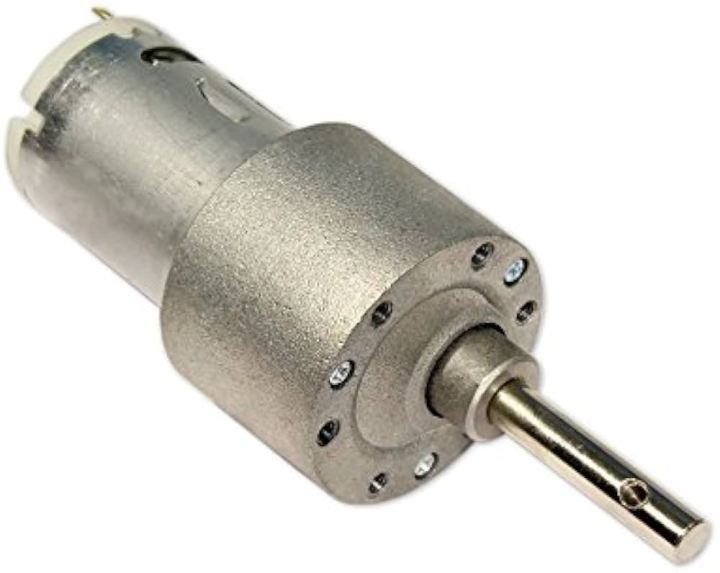
\includegraphics[width=0.5\textwidth]{3.1.jpg}
    \caption{Johnson Motor}
    \label{fig:3.1}
\end{figure}

\subsubsection*{3.1.2 Raspberry Pi 4}
Raspberry Pi 4 is a credit card-sized computer that can run an operating system and perform multiple functions. It is equipped with a Broadcom BCM2711, Quad core Cortex-A72 (ARM v8) 64-bit SoC @ 1.5GHz, 2GB RAM, and USB and HDMI ports. In this project, it processes voice commands, sends control signals to Arduino, and communicates with cloud services. [Source: \href{https://www.adafruit.com/product/4292}{Raspberry Pi 4 on Adafruit}]

\begin{figure}[H]
    \centering
    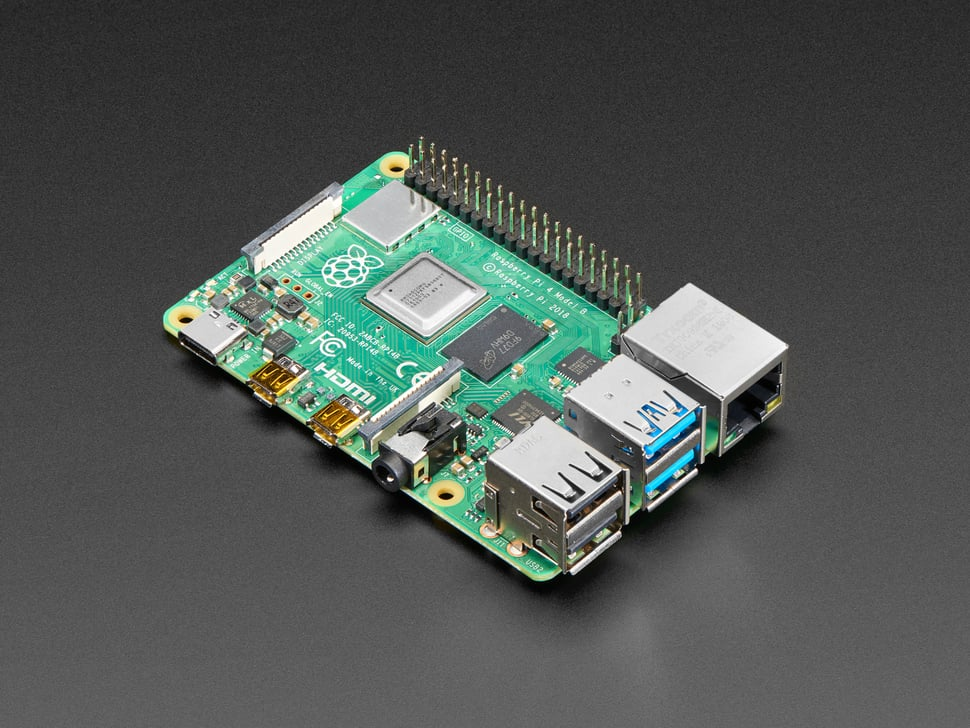
\includegraphics[width=0.5\textwidth]{fig3.2.jpg}
    \caption{Raspberry Pi 4}
    \label{fig:3.2}
\end{figure}

\subsubsection*{3.1.3 Arduino UNO}
The Arduino UNO is an open-source microcontroller board based on the Microchip ATmega328P microcontroller. It features 14 digital I/O pins, 6 analog inputs, a 16 MHz quartz crystal, and USB and power jack. In this project, it controls motors and sensors based on the instructions received from the Raspberry Pi. [Source: \href{https://digilog.pk/products/arduino-uno-kit-in-pakistan}{Arduino UNO on Digilog}]

\begin{figure}[H]
    \centering
    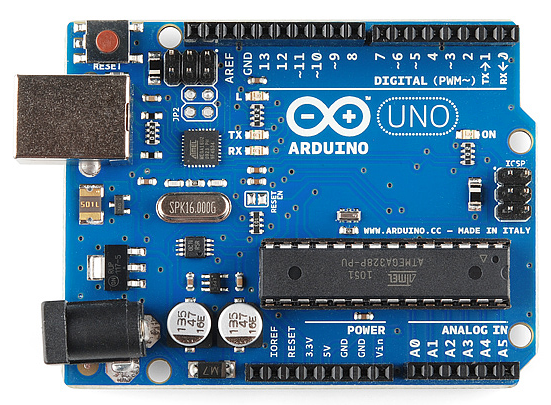
\includegraphics[width=0.5\textwidth]{fig3.3.png}
    \caption{Arduino UNO}
    \label{fig:3.3}
\end{figure}

\subsubsection*{3.1.4 IR Array Sensor}
IR (Infrared) array sensors are used to detect the path for line-following by emitting and detecting IR light. A group of IR sensors is arranged to detect black lines on a white surface. In this project, they help the robot follow the designated path. [Source: \href{https://www.giganepal.com/product/ir-sensor-array-module-4-way/?v=584a79c5e916}{IR Array Sensor on GigaNepal}]

\begin{figure}[H]
    \centering
    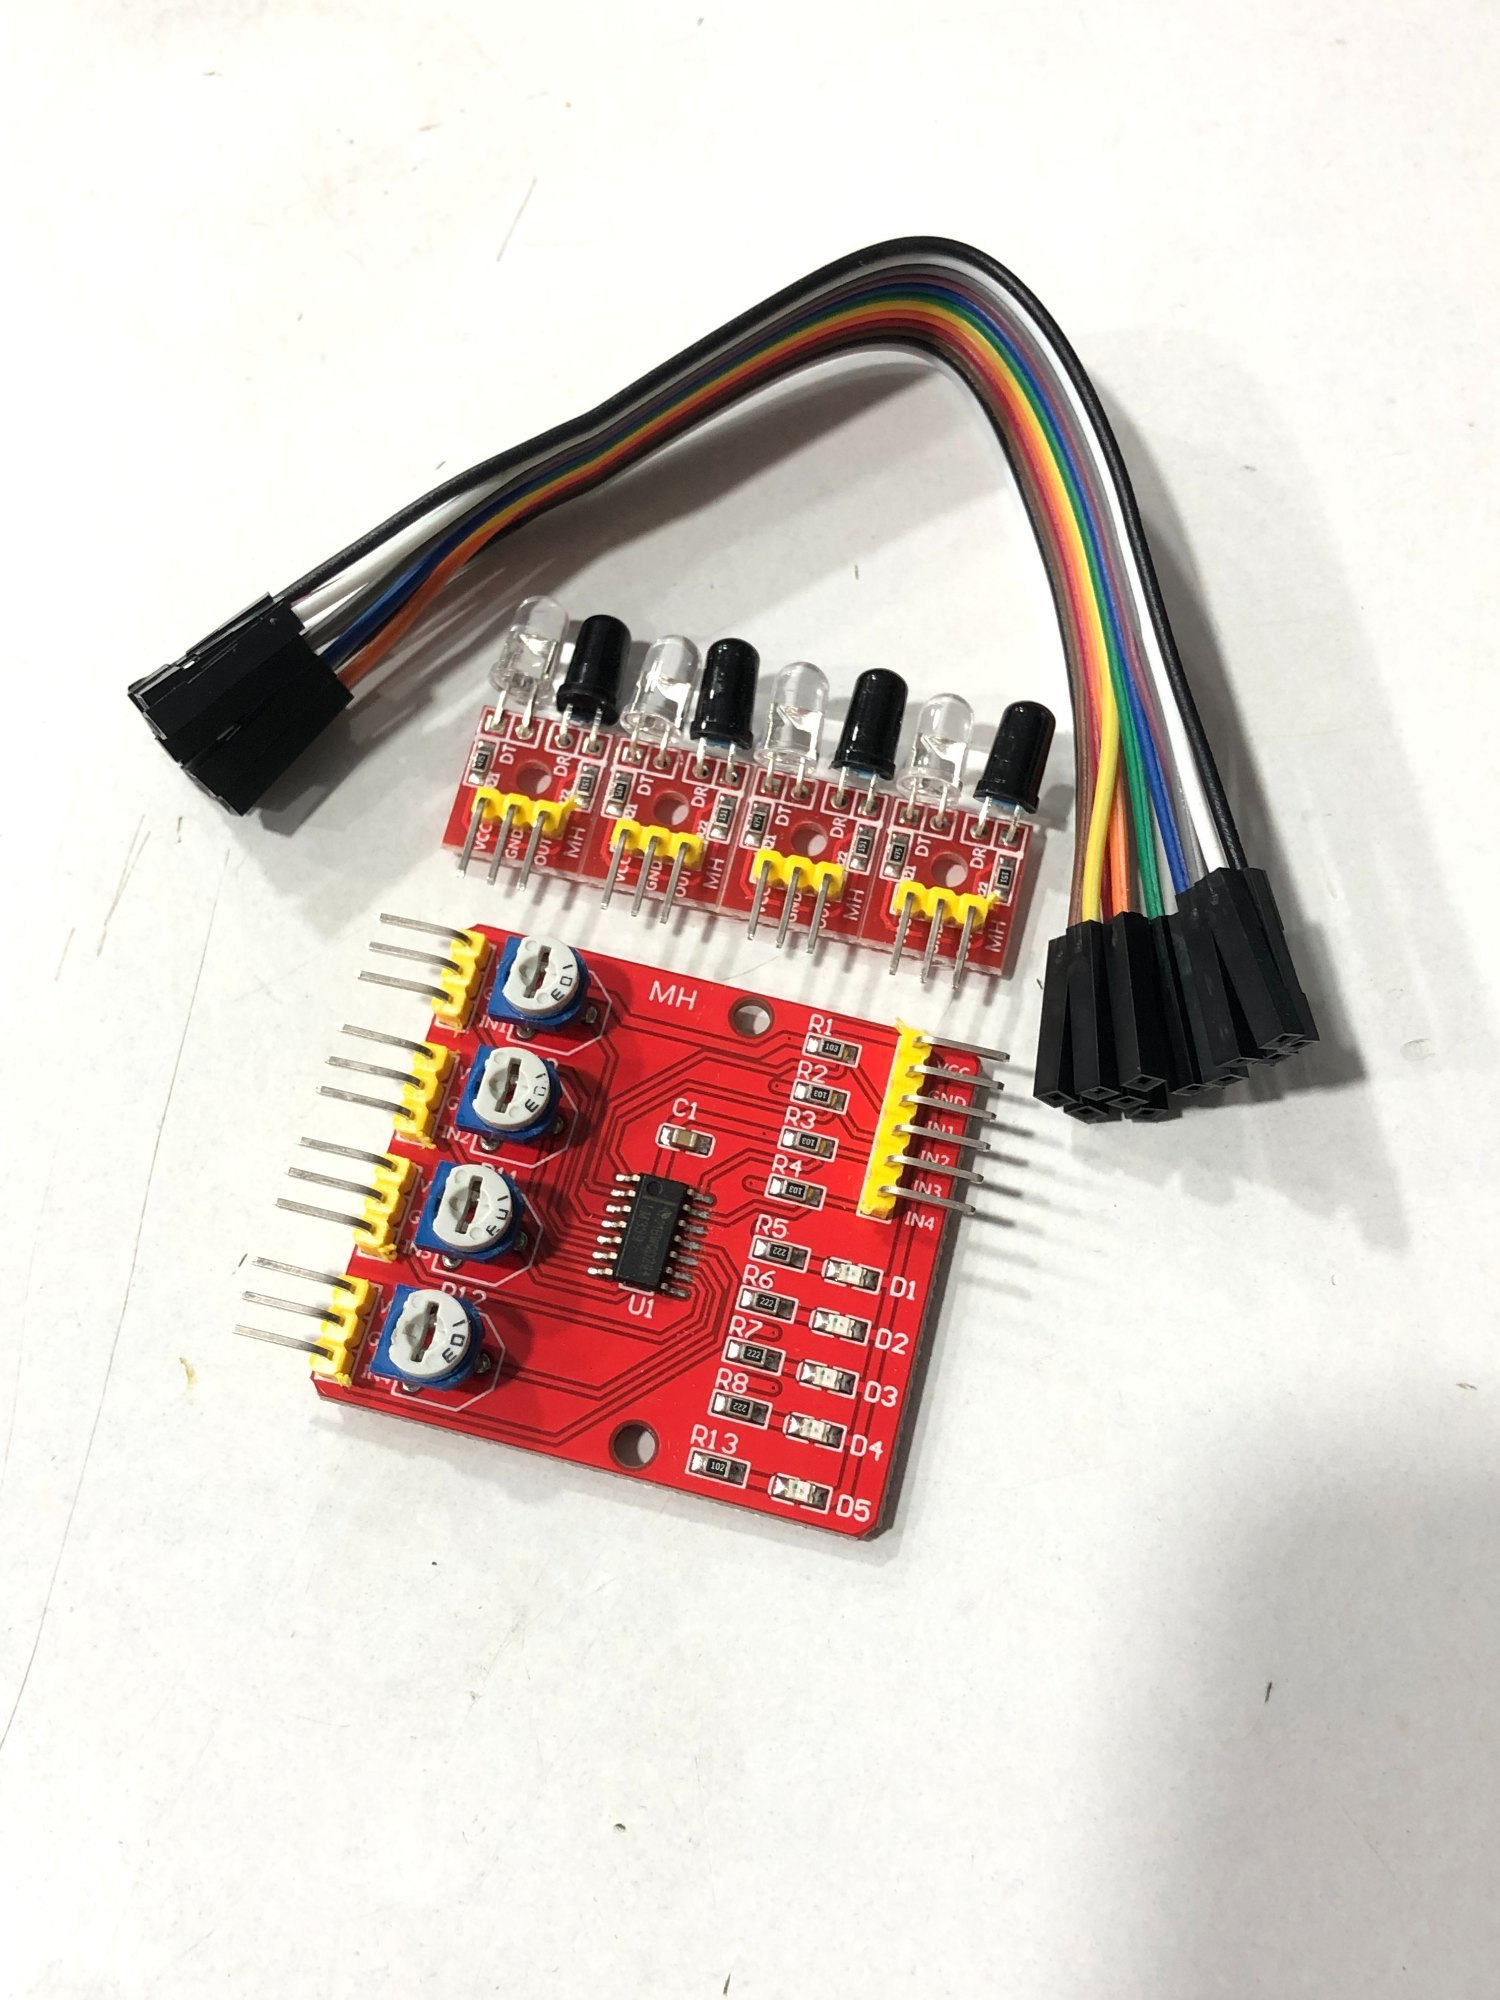
\includegraphics[width=0.5\textwidth]{3.4.jpg}
    \caption{IR Array Sensor}
    \label{fig:3.4}
\end{figure}

\subsubsection*{3.1.5 Metal Gear Servo MG996R}
The MG996R is a high-torque servo motor with metal gears and digital control. It provides accurate angle control and is used in the pill dispensing mechanism. It can rotate 0–180 degrees and is known for durability and stability. [Source: \href{https://www.waveshare.com/mg996r-servo.htm}{MG996R Servo on Waveshare}]

\begin{figure}[H]
    \centering
    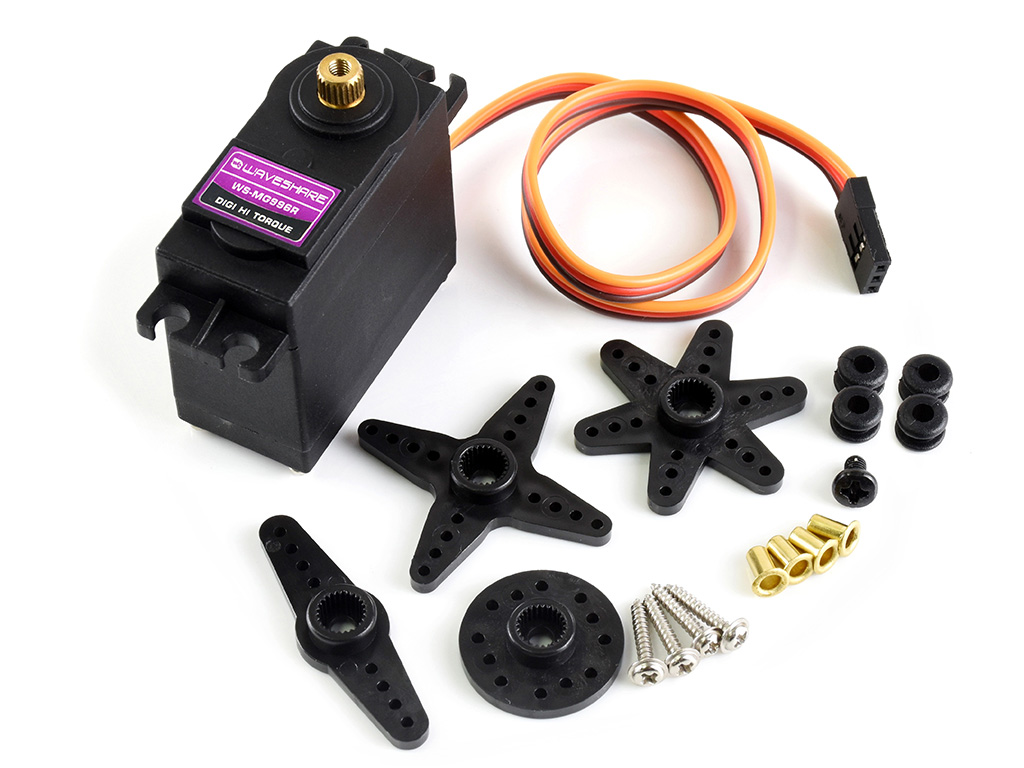
\includegraphics[width=0.5\textwidth]{3.5.jpg}
    \caption{Metal Gear Servo MG996R}
    \label{fig:3.5}
\end{figure}


\chapter{Feasibility Study}
\label{feasiblity}
\section{Technical Feasibility}

The project demonstrates strong technical feasibility by integrating robotics, automation, computer vision, and embedded systems in a practical and structured manner. The robot follows a modular design approach, dividing the system into three distinct compartments—bottom for motion, middle for storage, and top for pill dispensing—facilitating easier development, testing, and maintenance.

The bottom compartment handles mobility and line-following functionality, employing square DC geared motors that provide stable torque and compact integration within the chassis. Line-following is achieved through an array of IR sensors, managed by an Arduino Mega, which offers ample processing power and I/O ports to interface with motor drivers (e.g., L298N), sensor inputs, and communication modules.

The top compartment incorporates a Raspberry Pi equipped with a camera module for real-time patient recognition via facial recognition. This high-level processing unit manages time-based scheduling and activates a servo-driven pill dispensing mechanism based on the patient’s identity and medication schedule. A Real-Time Clock (RTC) module ensures accurate timing even during power fluctuations.

Communication between the Arduino and Raspberry Pi is established via UART or I2C protocols, enabling smooth coordination between navigation and pill dispensing functions. Wi-Fi modules (ESP8266/ESP32) are included for cloud integration, data logging, and alerts to healthcare personnel.

The system processes sensor data and camera inputs to make real-time decisions. Facial recognition utilizes open-source Python libraries such as OpenCV and \texttt{face\_recognition}, while the Arduino manages real-time control using standard libraries.

The modular hardware design ensures flexibility for part replacement, independent testing of sections, and future upgrades. The square motors offer robust and efficient movement, well-suited for indoor hospital or hostel environments. Overall, the project stands out for its adaptability, structured architecture, cost-effective components, and scalability, making it a technically feasible and reliable solution.

\section{Economic Feasibility}

The proposed system exhibits strong economic feasibility through a cost-effective approach to hardware development and deployment. Most required components—such as the Arduino, Raspberry Pi, IR sensors, servo motors, and square DC motors—are readily available in local electronics markets and commonly stocked in standard college laboratories. These components are significantly more affordable compared to commercial healthcare robots, making the system accessible for educational and research use.

Open-source platforms like the Arduino IDE and Python-based tools including OpenCV and \texttt{face\_recognition} eliminate the need for expensive proprietary software, substantially reducing development costs. Additionally, 3D printing parts using PLA filament allows low-cost prototyping and quick design iterations, enabling multiple refinements without heavy financial burden.

The project’s modular design supports incremental development—each compartment (movement, storage, dispensing) can be developed and tested separately, which spreads financial investment over time and improves budget management. Many components can be reused or repurposed during testing and final deployment, maximizing resource efficiency.

Further savings come from leveraging existing college infrastructure, such as power supplies, testing equipment, and computer systems, alongside the technical expertise of the team, which minimizes or eliminates external consultancy or training expenses.

In summary, the use of affordable, off-the-shelf components, open-source software, and in-house prototyping ensures strong economic viability. The scalable and adaptable design makes this solution ideal for healthcare automation in resource-constrained environments like government hospitals and orphanages.


\chapter{Methodology}
\label{methodology}
\section{Flowcharts}

\subsection{Overall System Workflow}

\tikzstyle{startstop} = [rectangle, rounded corners, minimum width=3cm, minimum height=1cm, text centered, draw=black, fill=white]
\tikzstyle{process} = [rectangle, minimum width=3.2cm, minimum height=1cm, text centered, draw=black, fill=white]
\tikzstyle{decision} = [diamond, aspect=2, minimum width=3.5cm, minimum height=1cm, text centered, draw=black, fill=white]
\tikzstyle{arrow} = [thick,->,>=stealth]

\begin{figure}[H]
\centering
\resizebox{\textwidth}{!}{ % scales to page width
\begin{tikzpicture}[node distance=1.5cm and 2.5cm]

% Main vertical nodes
\node (start) [startstop] {System Start};
\node (init) [process, below of=start] {Initialize RPi \& Arduino};
\node (nav) [process, below of=init] {Start Line Following};
\node (zone) [decision, below of=nav, yshift=-0.5cm] {Reached Patient Zone?};

% Yes branch (right)
\node (capture) [process, right=4cm of zone] {Capture Face Image};
\node (match) [process, below of=capture] {Facial Recognition};
\node (verify) [process, below of=match] {Verify Schedule (RTC)};
\node (dispense) [process, below of=verify] {Dispense Medication};
\node (log) [process, below of=dispense] {Log Data \& Notify};
\node (continue) [process, below of=log] {Continue/Return to Base};
\node (end) [startstop, below of=continue] {System End};

% No branch (left)
\node (move) [process, left=4cm of zone] {Move to Another Patient};

% Arrows - main flow
\draw [arrow] (start) -- (init);
\draw [arrow] (init) -- (nav);
\draw [arrow] (nav) -- (zone);

% Yes path
\draw [arrow] (zone.east) -- node[above] {Yes} (capture.west);
\draw [arrow] (capture) -- (match);
\draw [arrow] (match) -- (verify);
\draw [arrow] (verify) -- (dispense);
\draw [arrow] (dispense) -- (log);
\draw [arrow] (log) -- (continue);
\draw [arrow] (continue) -- (end);

% No path
\draw [arrow] (zone.west) -- node[above] {No} (move.east);
\draw [arrow] (move) |- (nav.west);

\end{tikzpicture}
}
\caption{Overall System Workflow}
\label{fig:overall_system_workflow}
\end{figure}


\subsection{Pill Dispensing Subsystem}

\begin{figure}[H]
\centering
\begin{tikzpicture}[node distance=1.5cm and 3cm]

\node (start) [startstop] {At Patient Zone};
\node (face) [process, below of=start] {Face Recognition};
\node (match) [decision, below of=face, yshift=-0.5cm] {Face Recognized?};
\node (check) [process, right of=match, xshift=5cm] {Check Schedule};
\node (abort) [process, left of=match, xshift=-5cm] {Abort \& Log};
\node (endAbort) [startstop, below of=abort] {Subsystem End};
\node (dispense) [process, below of=check] {Activate Servo \& Dispense};
\node (log) [process, below of=dispense] {Log Success};
\node (end) [startstop, below of=log] {Subsystem End};

\draw [arrow] (start) -- (face);
\draw [arrow] (face) -- (match);
\draw [arrow] (match.east) -- (check.west) node[midway, above] {Yes};
\draw [arrow] (match.west) -- (abort.east) node[midway, above] {No};
\draw [arrow] (abort) -- (endAbort);
\draw [arrow] (check) -- (dispense);
\draw [arrow] (dispense) -- (log);
\draw [arrow] (log) -- (end);

\end{tikzpicture}
\caption{Pill Dispensing Subsystem Flowchart}
\label{fig:pill_dispensing_subsystem}
\end{figure}


\subsection{Navigation and Obstacle Handling}

\begin{figure}[H]
\centering
\begin{tikzpicture}[node distance=1.5cm and 3cm]

\node (start) [startstop] {Start Line Following};
\node (read) [process, below of=start] {Read IR Sensor Data};
\node (pid) [process, below of=read] {PID-based Motor Control};
\node (obstacle) [decision, below of=pid, yshift=-0.5cm] {Obstacle Detected?};
\node (stop) [process, left of=obstacle, xshift=-5cm] {Stop \& Wait};
\node (endStop) [startstop, below of=stop] {Navigation End};
\node (move) [process, right of=obstacle, xshift=5cm] {Continue to Next Zone};
\node (endMove) [startstop, below of=move] {Navigation End};

\draw [arrow] (start) -- (read);
\draw [arrow] (read) -- (pid);
\draw [arrow] (pid) -- (obstacle);
\draw [arrow] (obstacle.west) -- (stop.east) node[midway, above] {Yes};
\draw [arrow] (obstacle.east) -- (move.west) node[midway, above] {No};
\draw [arrow] (stop) -- (endStop);
\draw [arrow] (move) -- (endMove);

\end{tikzpicture}
\caption{Navigation and Obstacle Handling Flowchart}
\label{fig:navigation_obstacle_handling}
\end{figure}


\chapter{Expected Output}
\label{result}
\begin{itemize}
    \item \textbf{Autonomous Line Following and Navigation:} \\
    The system will accurately follow predefined paths using IR sensor arrays, with a line detection accuracy of over 95\% on high-contrast surfaces. The square DC geared motors, controlled by an Arduino Mega, will ensure smooth and stable movement across hospital or hostel corridors. The robot will maintain a consistent speed suitable for indoor navigation (approx. 0.3–0.5 m/s), with minimal deviation from the line path even at junctions and turns.

    \item \textbf{Scheduled Pill Dispensing with Patient Recognition:} \\
    The top-mounted camera module, connected to the Raspberry Pi, will perform real-time facial recognition of patients using trained models with an expected accuracy of over 90\% in well-lit environments. Based on patient identity and the stored schedule, the system will trigger the appropriate servo motor to dispense the correct dosage from the designated pill compartment. The dispensing process will be completed within 3–5 seconds of successful identification.

    \item \textbf{Modular Operation and System Feedback:} \\
    Each compartment of the bot will operate semi-independently under a unified control system. The Raspberry Pi and Arduino will communicate via serial protocol to synchronize motion with dispensing operations. The system will provide LED or sound-based feedback for key actions—such as arrival at a patient’s bed, successful identification, and pill dispensing—ensuring operational transparency.

    \item \textbf{Real-Time Processing and Minimal Latency:} \\
    The facial recognition and pill dispensing processes will maintain a latency of under 1 second, ensuring quick and reliable patient interactions. The line-following subsystem will update motor commands at over 50 Hz, providing responsive and accurate path tracking. Power-efficient components will enable up to 1–2 hours of autonomous operation on a single battery charge, depending on the load.

    \item \textbf{Scalable and Adaptable Framework:} \\
    The modular design allows for easy expansion—additional compartments or storage trays can be added for more patients or different types of medicines. The robot can also be reprogrammed to follow new routes or modified to integrate RFID or QR code-based patient recognition as future enhancements.
\end{itemize}



\chapter*{Gantt Chart}
\addcontentsline{toc}{chapter}{Gantt Chart}
\label{ganttchart}
\begin{center}
\resizebox{\textwidth}{!}{%
\begin{ganttchart}[
    hgrid,
    vgrid,
    time slot format=isodate-yearmonth,
    time slot unit=month,
    x unit=1.6cm,
    y unit chart=1.6cm,
    y unit title=1cm,
    title height=1,
    bar height=0.6,
    bar/.append style={fill=blue!50},
    group right shift=0,
    group top shift=0.4,
    group height=.3,
    bar label font=\normalsize,
    bar label node/.append style={align=left, text width=4cm},
    group label node/.append style={align=left, text width=4cm}
]{2025-05}{2026-04}
    \gantttitlecalendar{year, month=shortname} \\

    % Project Phases
    \ganttbar[bar/.append style={fill=gray!70}]{Project Initiation}{2025-05-01}{2025-08-15} \\
    \ganttbar[bar/.append style={fill=gray!50}]{Research \& Requirements}{2025-05-15}{2025-09-15} \\
    \ganttbar[bar/.append style={fill=gray!50}]{Design}{2025-07-01}{2025-09-30} \\
    \ganttbar[bar/.append style={fill=gray!50}]{Software \& Simulation}{2025-09-01}{2026-04-30} \\
    \ganttbar[bar/.append style={fill=gray!70}]{Hardware Assembling}{2025-09-15}{2026-04-30} \\
    \ganttbar[bar/.append style={fill=gray!50}]{Documentation}{2025-06-01}{2026-04-30}
\end{ganttchart}%
}
\end{center}


\chapter*{Cost Estimation}
\addcontentsline{toc}{chapter}{Cost Estimation}
\label{cost estimation}
\section*{Components and Cost Distribution}

\begin{table}[h]
\centering
\small  % Shrinks font size just for this table
\renewcommand{\arraystretch}{1.05}  % Reduces row spacing
\resizebox{\textwidth}{!}{ % scales to page width
\begin{tabular}{|c|p{4.6cm}|c|r|r|p{3cm}|c|}
\hline
\textbf{S.N} & \textbf{Components} & \textbf{Qty} & \textbf{Unit Price (NRs)} & \textbf{Total Price (NRs)} & \textbf{Availability} & \textbf{In College} \\
\hline
1  & Johnson Motor Metal Gear 300rpm & 4 & 1,795 & 7,180 & Daraz Nepal & Yes \\\hline
2  & Raspberry Pi 3 (4GB RAM) & 1 & 13,000 & 13,000 & Technova & Yes \\\hline
3  & Raspberry Pi Camera Module (5MP) & 1 & 900 & 900 & Himalayan Solutions & Yes \\\hline
4  & LiPo Battery 2200mAh 3S 35C 11.1V & 2 & 2,000 & 4,000 & Technova & Yes \\\hline
5  & Arduino UNO  & 1 & 1,300 & 1,300 & Technova & Yes \\\hline
6  & Monster Motor Shield (VNH2SP30 30A) & 1 & 1,500 & 1,500 & GigaNepal & No \\\hline
7  & IR Sensor Array Module – 4 Way & 2 & 235 & 470 & GigaNepal & No \\\hline
8  & PLA Filament (2kg) & 1 & 6,000 & 6,000 & Daraz Nepal & No \\\hline
9  & Metal Gear Servo MG995 & 6 & 800 & 4,800 & Daraz Nepal & Yes \\\hline
10 & 16-Channel PCA9685 PWM Servo Driver & 1 & 330 & 330 & Daraz Nepal & No \\\hline
11 & Robot Wheel (10cm × 4cm) & 4 & 275 & 1,100 & Supreme Light & Yes \\\hline
12 & Connecting Wires (M-M, M-F, F-F) & 40 & 900 & 900 & Daraz Nepal & No \\\hline
13 & LiPo IMAX B6 Battery Charger & 1 & 3,940 & 3,940 & Daraz Nepal & Yes \\\hline
14 & 0.96" OLED Display & 1 & 600 & 600 & GigaNepal & No \\\hline
15 & 12mm Piezo Buzzers (5V, 2pcs) & 1 & 70 & 70 & GigaNepal & Yes \\\hline
16 & Buck Converter (LM2596) & 1 & 180 & 180 & Technova & Yes \\\hline
17 & Soldering Wire & 1 & 120 & 120 & GigaNepal & No \\\hline
18 & SD Card 32GB & 1 & 700 & 700 & Daraz & No \\\hline
19 & Arduino Connector (5M) & 1 & 100 & 100 & Technova & No \\\hline
20 & Bread Board(400 pts) & 1 & 120 & 120 & Daraz & Yes \\\hline
21 & Matrix Board(400 pts) & 2 & 45  & 90 & Daraz & Yes \\\hline
22 & 3D printing cost & 1 & 5,000  & 5,000 & 3d Khet & No \\
\hline
\multicolumn{4}{|r|}{\textbf{Total Cost}} & \multicolumn{3}{l|}{\textbf{NRs. 52,400}} \\
\hline
\multicolumn{4}{|r|}{\textbf{Total Cost (Not Available In College)}} & \multicolumn{3}{l|}{\textbf{NRs. 15,720}} \\
\hline
\end{tabular}
}
\caption{Components, Cost Distribution, Availability, and In College Status}
\end{table}



\chapter*{References}
\addcontentsline{toc}{chapter}{References}
\label{references}
\begin{thebibliography}{99}
  \bibitem{1} R. Sharma and S. Mehta, “Design of a line-following robot...”
  \bibitem{2} D. Patel and A. Verma, "Design and Implementation of a Modular Hospital Delivery Robot..."
  \bibitem{3} Y. Kim, H. Lee, and J. Park, “PillGood: Automated and Interactive Pill Dispenser...”
  \bibitem{4} L. Basyal, “Efficient Human Identification Through Face Detection...”
  \bibitem{5} A. Jabeena et al., “Automatic Pill Reminder for Easy Supervision...”
  \bibitem{6} S. Sawargaonkar et al., “Multipurpose Tray with an Extendable Holder...”
  \bibitem{7} Johnson Motor Metal Gear 300RPM. [Online]. Available: \url{https://www.daraz.com.np/products/johnson-motor-metal-gear-300rpm-i129797381.html}
  \bibitem{8} Raspberry Pi 4 on Adafruit. [Online]. Available: \url{https://www.adafruit.com/product/4292}
  \bibitem{9} Arduino UNO on Digilog. [Online]. Available: \url{https://digilog.pk/products/arduino-uno-kit-in-pakistan}
  \bibitem{10} IR Sensor Array Module 4-Way on GigaNepal. [Online]. Available: \url{https://www.giganepal.com/product/ir-sensor-array-module-4-way/?v=584a79c5e916}
  \bibitem{11} MG996R Servo on Waveshare. [Online]. Available: \url{https://www.waveshare.com/mg996r-servo.html}
\end{thebibliography}

%\bibliographystyle{plain} % or another style like ieee, unsrt, etc.
%\bibliography{references} % references.bib (no .bib extension)


\end{document}
